% Generated by experiments/make_figures.py.
\definecolor{cA}{HTML}{2a78d6}\definecolor{cB}{HTML}{eb6834}\definecolor{cC}{HTML}{1baf7a}%
\definecolor{cD}{HTML}{4a3aa7}\definecolor{cGray}{HTML}{8a8984}%
\definecolor{lvA}{HTML}{c6dbf5}\definecolor{lvB}{HTML}{93bbec}\definecolor{lvC}{HTML}{5e98e0}%
\definecolor{lvD}{HTML}{2a78d6}\definecolor{lvE}{HTML}{174a8c}\definecolor{lvF}{HTML}{1baf7a}%
\begin{figure}
  \centering
  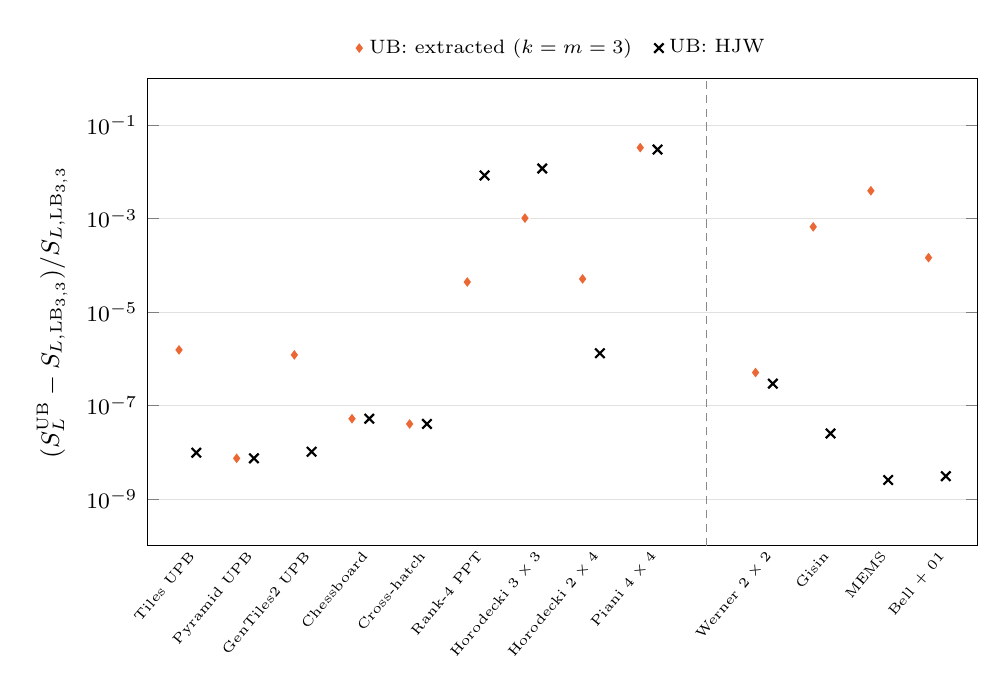
\begin{tikzpicture}
    \begin{axis}[width=\columnwidth, height=0.62\columnwidth, ymode=log, ymin=1e-10, ymax=1,
      ylabel={$(S_L^{\mathrm{UB}}-S_{L,\mathrm{LB}_{3,3}})/S_{L,\mathrm{LB}_{3,3}}$},
      xtick={1,2,3,4,5,6,7,8,9,11,12,13,14}, xticklabels={{Tiles UPB},{Pyramid UPB},{GenTiles2 UPB},{Chessboard},{Cross-hatch},{Rank-4 PPT},{Horodecki $3\times3$},{Horodecki $2\times4$},{Piani $4\times4$},{Werner $2\times2$},{Gisin},{MEMS},{Bell + $\ket{01}$}}, xmin=0.30000000000000004, xmax=14.7,
      xticklabel style={rotate=50, anchor=north east, font=\tiny, inner sep=1pt}, tick label style={font=\footnotesize},
      label style={font=\small}, legend style={font=\scriptsize, at={(0.5,1.02)}, anchor=south, draw=none,
      legend columns=2, /tikz/every even column/.append style={column sep=6pt}}, legend cell align=left,
      ymajorgrids, grid style={cGray!25},
      xtick style={draw=none}]
            \addplot[only marks, mark=diamond*, mark size=2.2pt, cB, mark options={draw=white, line width=0.4pt}] coordinates {(0.85,1.5515e-06) (1.85,7.43795e-09) (2.85,1.21318e-06) (3.85,5.23793e-08) (4.85,4.04678e-08) (5.85,4.41014e-05) (6.85,0.00102322) (7.85,5.12697e-05) (8.85,0.0329973) (10.85,5.09192e-07) (11.85,0.000667107) (12.85,0.0039366) (13.85,0.00014604)};\addlegendentry{UB: extracted ($k=m=3$)}
      \addplot[only marks, mark=x, mark size=2.4pt, black, thick] coordinates {(1.15,9.80612e-09) (2.15,7.43801e-09) (3.15,1.03007e-08) (4.15,5.24118e-08) (5.15,4.0468e-08) (6.15,0.00838827) (7.15,0.0118261) (8.15,1.31759e-06) (9.15,0.0300567) (11.15,2.94112e-07) (12.15,2.53659e-08) (13.15,2.55743e-09) (14.15,3.08745e-09)};\addlegendentry{UB: HJW}
      \draw[cGray, densely dashed] (axis cs:10,1e-10) -- (axis cs:10,1);
    \end{axis}
  \end{tikzpicture}
  \caption{Relative gap between the upper bounds on $\widehat{S_L}$ and the SDP lower bound at $k=m=3$, for the
  states of Fig.~\ref{fig:namedLinearEntropy} (PPT left of the dashed line, NPT right). Orange: decomposition
  extracted from the SDP solution (Sec.~\ref{sec:extractingTheDecomposition}); black: HJW gradient descent from
  random starts. Points at $10^{-10}$ are gaps below solver precision.}
  \label{fig:upperBounds}
\end{figure}
